\documentclass{handout}

\SetInstructor{Lt Col James Phillips}
\SetCourseTitle{ECE231: Electrical Circuits and Systems I}
\SetSemester{Spring 2016}
\SetHandoutTitle{Lecture 17: Operational Amplifiers - Part 4: Instrumentation Systems}

%\SetDueDate{1 Jan 2016}
%\ShowAllBlanks

\showsoln \setsolncolor{red}

\begin{document}
\maketitle

\textbf{Upcoming events}
\begin{enumerate}
\item HW \#4 due TODAY
\item Problem Set \#3 due next lesson
\item Quiz \#3 during next lesson
\item Problem Set \# 4 due Lesson 23
\item HW \# 5 due Lesson 25
\item Problem Set \# 5 due Lesson 25
\item Quiz 4 Lesson 26
\end{enumerate}

\textbf{OBJECTIVES:}
\begin{enumerate}
\item Understand the purpose of transducers and instrumentation systems
\item Calculate gain and bias for instrumentation systems and implement with Op Amps
\end{enumerate}

\textbf{READING}
\begin{description}
\item [Required]:
\begin{itemize}
\item  Textbook, section 4.6, pages 211--223
\end{itemize}
\item [Optional]: None
\end{description}

\textbf{HOMEWORK}
\begin{description}
\item [Required textbook problems]: 4.64, 4.65--- Due Lesson 23
\item [Recommended textbook problems]: 4.63
\end{description}

\section{What is an Instrumentation System?}
\subsection{Transducers}
Before we can talk in detail about instrumentation systems, we have to talk about transducers.  What is a transducer?

\soln{1.5in}{
A transducer is a device that turns a physical signal into an electrical signal or vice versa.  There are two types
\begin{description}
\item[Input Transducers] turn a physical signal into an electrical signal
\item[Output Transducers] turn electrical signals to physical signals
\end{description}
We will assume our transducers have a linear response.
}

List some transducer examples:

\soln{3in}{
Input Transducers: Microphone, mouse/touchpad, keyboard, motion sensor, ....

Output Transducers: Computer display (monitor), speaker, Light bulb, .....
}

Input transducers are broken into two categories:
\begin{description}
\item[Active transducers] produce a voltage or current proportional to the physical parameter being measured (i.e. a piezo electric crystal in a bathroom scale)
\item[Passive transducers] do not produce a current or voltage, but rather change a parameter like resistance or conductance in proportion to the input being measured (i.e. a photo-resistor that changes resistance based on light falling on the photosensitive surface)
\end{description}

\subsection{Basic Instrumentation Systems}

More often than not, the range (magnitude and bias) of the signal from the input transducer is not appropriate to connect directly to a circuit or output transducer.  This is where instrumentation systems come in handy; you will sometime hear an instrumentation system referred to as a transducer interface.  Figure \ref{fig: InstrumentationSystem} shows a block diagram of a basic instrumentation system; you may hear me sometimes refer to this as a {\em fishbone diagram}.  

\begin{figure} [h!]
\centering
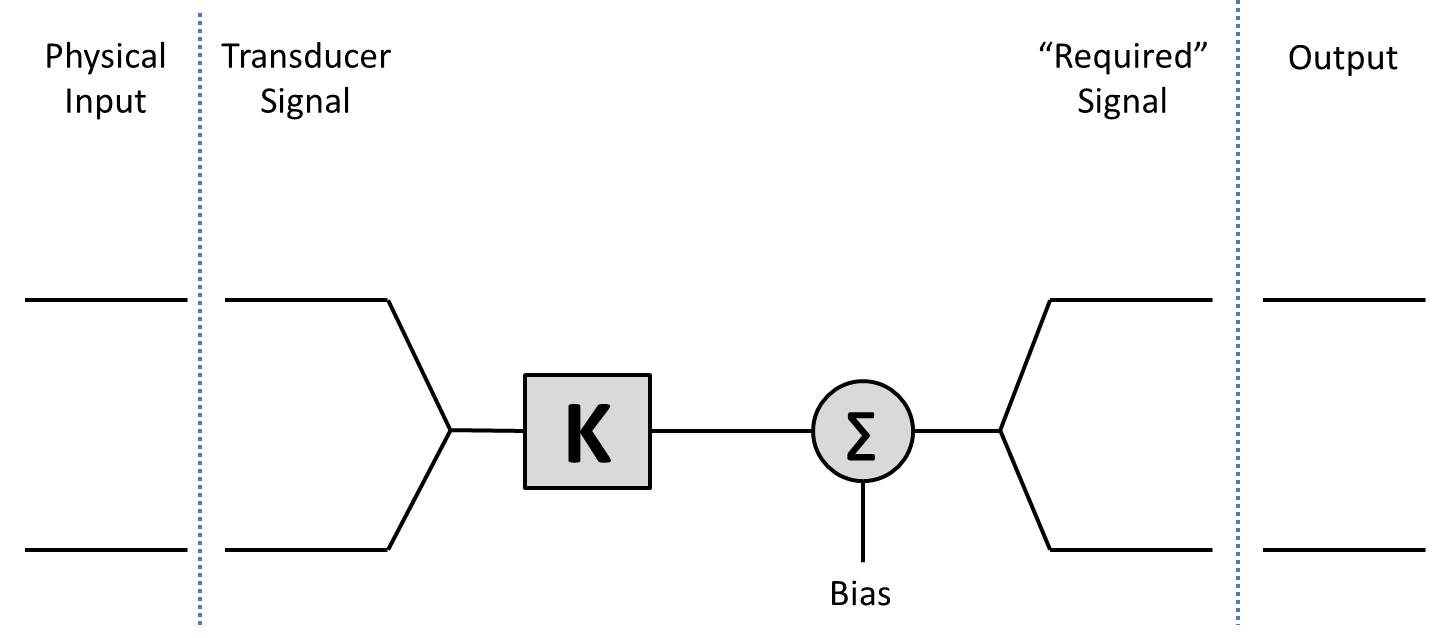
\includegraphics[width=0.75\textwidth]{InstrumentationSystem.jpg}
\caption{Basic Instrumentation System Diagram}
\label{fig: InstrumentationSystem}
\end{figure}
This system is shown broken into four parts:  
\soln{4in}{
\begin{description}
\item[Physical Input] is the physical value that the transducer is measuring (pressure, temperature, sound, etc.)
\item[Transducer Signal] is the electrical output of the input transducer (usually in volts or amps)
\item[``Required'' Signal] is the elctrical input required for the next stage of the system (a display for example)
\item[Ouput] should match the physical input value and is a good check to see that the system is configured properly.
\end{description}
}
Once we add the proper values onto the diagram, we can solve for the gain, $K$, and the bias.  Like most things this will make more sense when we do an example.
\newpage
\clearpage
\pagebreak
\textbf{Example 1}
The rudder control unit in an aircraft supplies a $-2.5\ mV$ signal when the pilot want full left rudder and a $2.5\ mV$ signal with the pilot wants full right rudder.  The rudder actuator requires $-5\ V$ for full left and $10\ V$ for full right.  Design an instrumentation system to allow this rudder system to work.
\soln{5in}{
\begin{figure} [h!]
\centering
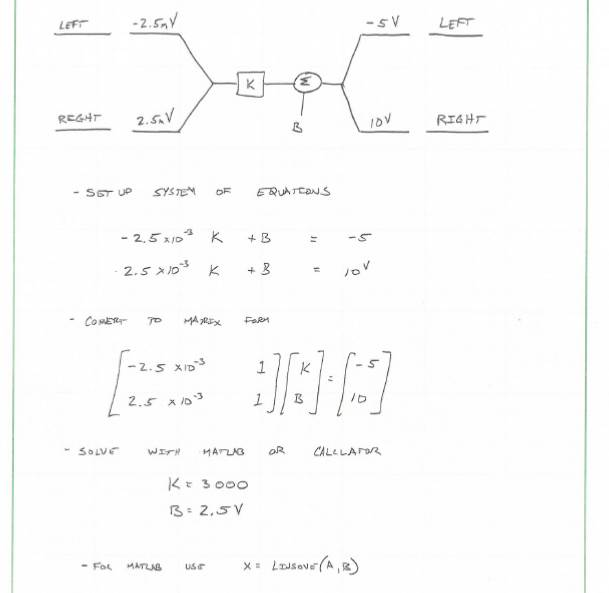
\includegraphics[width=1\textwidth]{Example1.jpg}
\end{figure}
}

\newpage
\clearpage
\pagebreak

\section{Building Instrumentation Systems with Op Amps}
Now that we understand how to find the required gain and bias of an instrumentation system, we need to learn to build these systems.  to do this we rely on our old friend the Op Amp.  

\textbf{Example 2}

In the way of a simple example, let's design an Op Amp circuit to implement the instrumentation system from example 1.  

\soln{7in}{
We can start by drawing a simplified block diagram: 
\begin{figure} [h!]
\centering
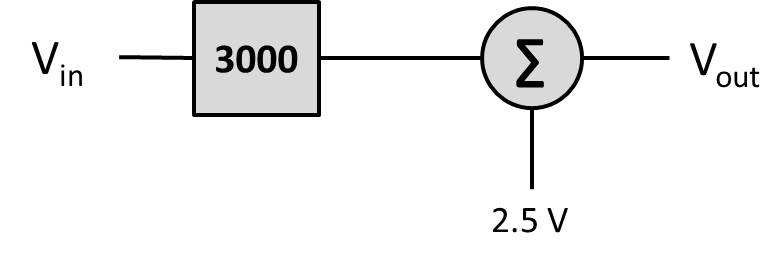
\includegraphics[width=0.4\textwidth]{Example1BlockDiagram.jpg}
\end{figure}

This is just the fishbone diagram without the ``wings'' on the input and output.  Since the system really only have one input and one output, this version of the block diagram more accurately represents the circuit we must build.

Now, let's write an equation for the transfer characteristic:
\begin{equation}
V_{out} = 3000V_{in} + 2.5V
\end{equation}

Since the gain on $V_{in}$ is large; we can split it into 2 gain stages

\begin{equation}
V_{out} = 150\times20\times V_{in} + 2.5V
\end{equation}

Allow me to modify this equation slightly
\begin{equation}
V_{out} = \left[-150\times -20\times V_{in} \right] +\left[ -5V \times -\frac{1}{2}\right]
\end{equation}

This gives us gains of $K_1 = -150$, $K_2=-20$ and $K_3 = -\frac{1}{2}$

We can implement this with an inverting amplifier followed by a weighted summer with one input connected to our negative power supply voltage ($-5\ V$):
\begin{figure} [h!]
\centering
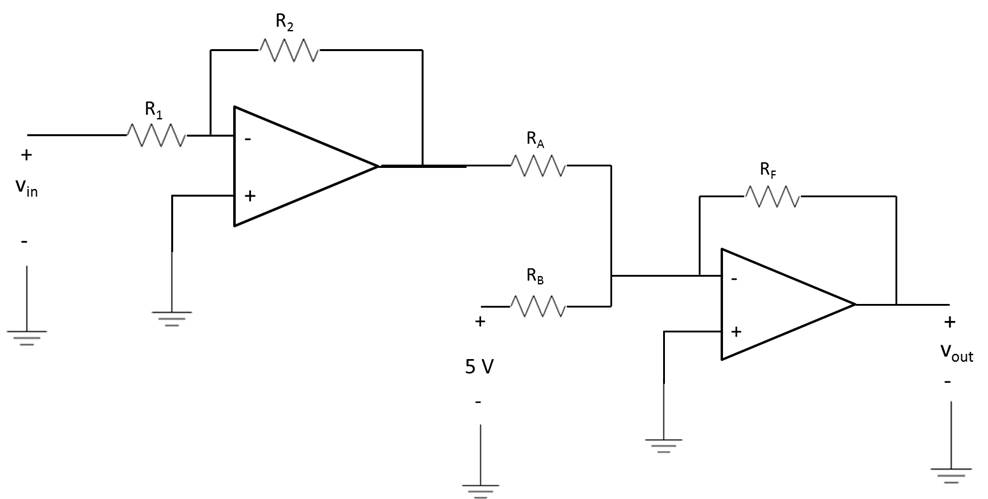
\includegraphics[width=0.7\textwidth]{Example2solnA.jpg}
\end{figure}

If we let $R_2 = 100\ k\Omega$ and $R_F = 100\ k\Omega$ we can calculate the other resistances:
\begin{eqnarray}
R_1 = -\frac{R_2}{K_1}=-\frac{100\ k\Omega}{-150} = 667\ \Omega \nonumber \\
R_A = -\frac{R_F}{K_2}=-\frac{100\ k\Omega}{-20} = 5\ k \Omega  \nonumber \\
R_B = -\frac{R_F}{K_3}=-\frac{100\ k\Omega}{0.5} = 200\ k \Omega \nonumber
\end{eqnarray} 

Note: You may consider buffering the inputs.  
}

\newpage
\clearpage
\pagebreak

\textbf{Example 3}

We have a pressure sensor whose input-output relationship is shown in Figure \ref{fig: Example3Graph}.  The sensor also has a Thevenin resistance of $R_T = 1\ k\Omega$.  We need to connect it to a meter that displays $-100\ psi$ when it receives a $-5\ V$ input and displays $1000\ psi$ when it receives a $5\ V$ input.  Design the appropriate instrumentation system using Op Amps.
\begin{figure} [h!]
\centering
\includegraphics[width=0.5\textwidth]{Example3Graph.jpg}
\caption{Pressure sensor input-output characteristic}
\label{fig: Example3Graph}
\end{figure}

\soln{6in}{
\begin{figure} [h!]
\centering
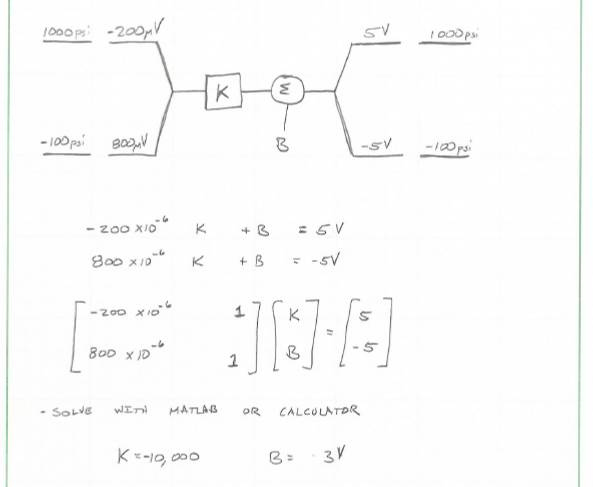
\includegraphics[width=0.8\textwidth]{Example3solnA.jpg}
\end{figure}
}

\newpage
\clearpage
\pagebreak

\soln{8in}{
\begin{figure} [h!]
\centering
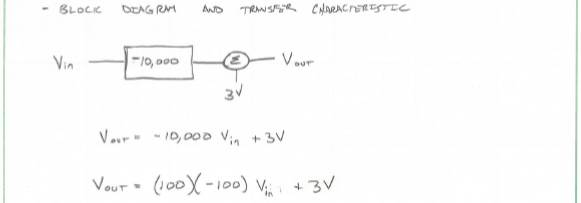
\includegraphics[width=0.8\textwidth]{Example3solnB.jpg}
\end{figure}

\begin{figure} [h!]
\centering
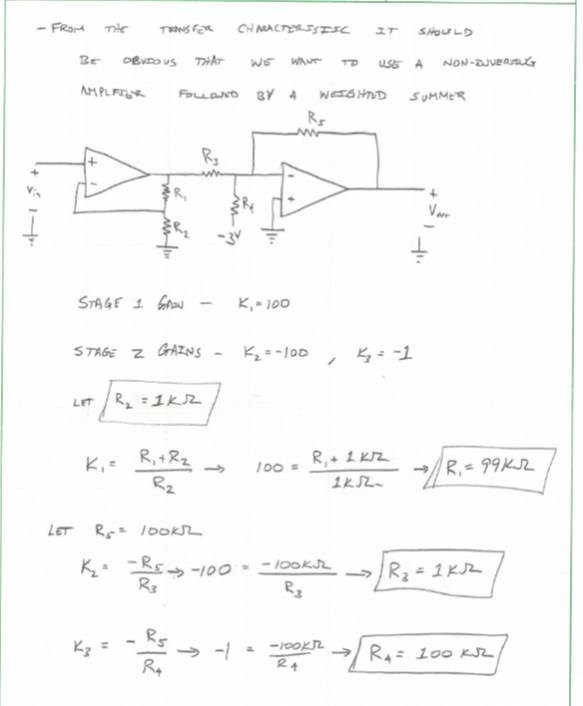
\includegraphics[width=0.8\textwidth]{Example3solnC.jpg}
\end{figure}
}

\newpage
\clearpage
\pagebreak

\end{document}


% Equation Array Example Code
%\begin
%{eqnarray}
%P_R &=& i_R^2R \nonumber \\
%P_R &=& (100\ mA)^2 \times 100\ \Omega \nonumber \\
%P_R &=& (100 \times 10^{-3}\ A)^2 \times 100\ \Omega \\
%P_R &=& 10000 \times 10^{-6}\ A^2  \times 100\ \Omega \nonumber \\
%P_R &=& 1\ W  \nonumber
%\end{eqnarray} 

% Figure Example Code
%\begin{figure} [h! t! b!]
%\centering
%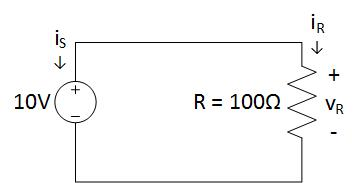
\includegraphics[width=0.5\textwidth]{OhmsLawExampleSolution.jpg}
%\caption{Ohm's Law example circuit}
%\label{fig: OhmsLawExampleSolution}
%\end{figure}

%Table Example Code
%\begin{table}[h]
%\centering
%\begin{tabular}{|l|c|c|}
%\hline
%Prefix & Abbreviation & Value \\
%\hline \hline
%Giga & $G$ & $10^9$ \\
%Mega & $M$ & $10^6$ \\
%Kilo & $k$ & $10^3$ \\
%\hline
%milli & $m$ & $10^{-3}$ \\
%micro & $\mu$ & $10^{-6}$ \\
%nano & $n$ & $10^{-9}$ \\
%pico & $p$ & $10^{-12}$ \\
%\hline
%\end{tabular}
%\caption{Engineering prefixes and values}
%\label{tab: Eng Prefixes}
%\end{table}
